\documentclass{standalone}
\usepackage{tikz}
\usetikzlibrary{positioning, calc, backgrounds, fit, shapes, shapes.multipart, shapes.symbols, backgrounds, fit}

\begin{document}
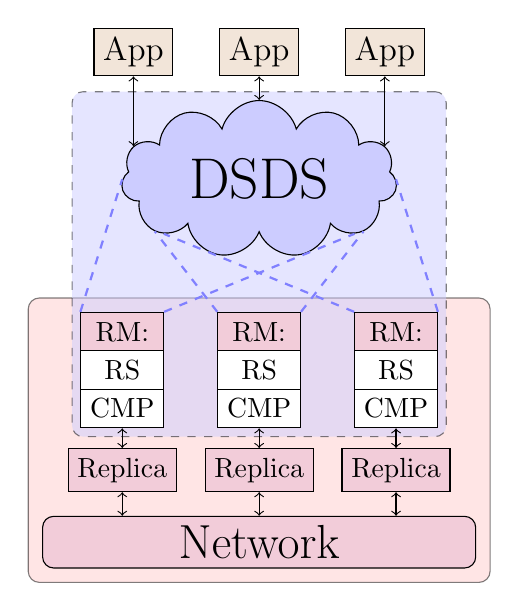
\begin{tikzpicture}[ 
    app/.style = {rectangle, draw, fill = brown!20, font = \large}, 
    rm/.style = {rectangle split, rectangle split parts = 3, rectangle split part fill = {purple!20, white, white}, draw},
    app-dsds/.style = {<->},
    mapping/.style = {dashed, thick, blue!50},
    replica/.style = {rectangle, draw, fill = purple!20},
    rm-replica/.style = {<->},
    network/.style = {rectangle, draw, fill = purple!20, rounded corners, minimum width = 5.5cm},
    mp/.style = {<->}]
  % dsds: distributed shared data service
  \node[name = dsds, cloud, cloud puffs = 11, draw, fill = blue!20, aspect = 3, minimum width = 3.50cm, minimum height = 2.00cm] {\huge DSDS};

  % apps
    % app1 above dsds.puff 1
  \node[app, above = 0.30cm of dsds.puff 1] (app1) {App};
    % app3 above dsds.puff 3
  \path let \p1 = (dsds.puff 3), \p2 = (app1) in node[app] (app3) at (\x1, \y2) {App};
    % app10 above dsds.puff 10
  \path let \p1 = (dsds.puff 10), \p2 = (app1) in node[app] (app10) at (\x1, \y2) {App};

  % apps <-> dsds
    % app1 <-> dsds.puff 1
  \draw[app-dsds] (app1) to (dsds.puff 1);
    % app3 <-> dsds.puff 3
  \draw[app-dsds] (app3) to (dsds.puff 3);
    % app10 <-> dsds.puff 10
  \draw[app-dsds] (app10) to (dsds.puff 10);

  % rm: replica manager
  \node[rm, below = of dsds.south] (rm-center) {RM: \nodepart{second} RS \nodepart{third} CMP};
    % rm-west below dsds.west
  \path let \p1 = (dsds.west), \p2 = (rm-center) in node[rm] (rm-west) at (\x1, \y2) {RM: \nodepart{second} RS \nodepart{third} CMP};
    % rm-east below dsds.east
  \path let \p1 = (dsds.east), \p2 = (rm-center) in node[rm] (rm-east) at (\x1, \y2) {RM: \nodepart{second} RS \nodepart{third} CMP};

  % rm -- dsds mapping
  \draw[mapping] (rm-west.north west) to (dsds.west);
  \draw[mapping] (rm-west.north east) to (dsds.south east);

  \draw[mapping] (rm-center.north west) to (dsds.puff 5);
  \draw[mapping] (rm-center.north east) to (dsds.puff 8);

  \draw[mapping] (rm-east.north west) to (dsds.south west);
  \draw[mapping] (rm-east.north east) to (dsds.east);

  % replica
  \node[replica, below = 0.25cm of rm-center] (replica-center) {Replica};
  \node[replica, below = 0.25cm of rm-west] (replica-west) {Replica};
  \node[replica, below = 0.25cm of rm-east] (replica-east) {Replica};

  % rm <-> replica
  \draw[rm-replica] (rm-center) to (replica-center);
  \draw[rm-replica] (rm-west) to (replica-west);
  \draw[rm-replica] (rm-east) to (replica-east);

  % network
  \node[network, below = 0.30cm of replica-center] (network) {\LARGE Network};

  % mp: message-passing
  \draw[mp] (replica-center) to (network);
  \draw[mp] (replica-west) to (replica-west |- network.north);
  \draw[mp] (replica-east) to (replica-east |- network.north);

  % mps-layer: message-passing system background including rm, replica, and network
  \begin{pgfonlayer}{background}
    \node[draw, fill = red!20, semitransparent, rectangle, rounded corners, inner sep = 5pt, fit = (rm-west) (rm-east) (network)] (mps-layer) {};
  \end{pgfonlayer}

  % dsds-layer: distributed shared data service including rm and dsds
  \begin{pgfonlayer}{background}
    \node[draw, fill = blue!20, semitransparent, rectangle, rounded corners, dashed, inner sep = 3pt, fit = (rm-west) (rm-east) (dsds)] (dsds-layer) {};
  \end{pgfonlayer}
\end{tikzpicture}
\end{document}
